%arara : pdflatex
\documentclass[12pt]{article}

\usepackage{../../TP0/style}

\begin{document}
\def\reportnumber{1}
\def\reporttitle{Étude expérimentale des Algorithmes de Tri.}
%----------------------------------------------------------------------------------------
%	TITLE PAGE
%----------------------------------------------------------------------------------------


\begin{titlepage} % Suppresses displaying the page number on the title page and the subsequent page counts as page 1
	\newcommand{\HRule}{\rule{\linewidth}{0.5mm}} % Defines a new command for horizontal lines, change thickness here
	
	\center % Centre everything on the page
	
	%------------------------------------------------
	%	Headings
	%------------------------------------------------
	
	\baselineskip=2\baselineskip 
	\textsc{\LARGE Université des Sciences et de la Technologie Houari Boumediene}%\\[1cm] % Main heading such as the name of your university/college

	%------------------------------------------------
	%	Logo
	%------------------------------------------------
	
	%\vfill\vfill
	\vfill
	
\includegraphics[width=0.3\textwidth]{../../TP0/USTHB_Logo.png}\\[1cm] % Include a department/university logo - this will require the graphicx package
	 
	%----------------------------------------------------------------------------------------
	
	\textsc{\Large Conception et Complexité des Algorithme}\\[0.5cm] % Major heading such as course name
	%\textsc{\large Minor Heading}\\[0.5cm] % Minor heading such as course title
	
	%------------------------------------------------
	%	Title
	%------------------------------------------------
	
	\HRule\\[0.4cm]
	\baselineskip=1.2\baselineskip 
	{\huge\bfseries Rapport de Travaux Pratiques N\textdegree  \reportnumber \\ \reporttitle}\\[0.4cm] % Title of your document
	
	\HRule\\[1.5cm]
	
	%------------------------------------------------
	%	Author(s)
	%------------------------------------------------
	
	\begin{minipage}{0.4\textwidth}
		\begin{flushleft}
			\large
			\textit{Binôme}\\
			MOHAMMEDI \textsc{Haroune } % Your name
			\\
			HOUACINE  \textsc{Naila Aziza} % Your name
		\end{flushleft}
	\end{minipage}
	~
	\begin{minipage}{0.4\textwidth}
		\begin{flushright}
			\large
			\textit{Professeur}\\
			Pr. AMANI \textsc{Ferhat} % Supervisor's name
		\end{flushright}
	\end{minipage}
	
	%------------------------------------------------
	%	Date
	%------------------------------------------------
	
	\vfill\vfill\vfill % Position the date 3/4 down the remaining page
	
	{\large\today} % Date, change the \today to a set date if you want to be precise
	
	
	\vfill % Push the date up 1/4 of the remaining page
	
\end{titlepage}



\tableofcontents
\setcounter{tocdepth}{2}

\newpage

\section{Notions générales.}
\subsection{Diviser pour régner!}
Les algorithmes qui suivent généralement l'approche dite "diviser pour régner" séparent le problème en plusieurs sous-problèmes semblables au problème initial mais de taille moindre, résolvent les sous-problèmes de façon récursive, puis combinent toutes les solutions pour produire la solution du problème original.
L'un des avantages des algorithmes "diviser-pour-régner" est que leurs temps d'exécution sont souvent faciles à déterminer.
Le paradigme "diviser-pour-régner" implique trois étapes à chaque niveau de la récursivité :
    Diviser : le problème en un certain nombre de sous-problèmes.
    Régner : sur les sous-problèmes en les résolvant de manière récursive. Si la taille d'un sous-problème est suffisamment réduite, on peut toutefois le résoudre directement.
    Combiner : les solutions des sous-problèmes pour produire la solution du problème original.
    
\subsection{Qu'est ce qu'un tas ?}
Un tas est une structure de données de type arbre, tel que ses clés sont ordonnées selon la propriété de tas : la clé d'un nœud parent a une plus haute priorité que les clés de ses enfants.\\
 La "priorité" signifie ici que les clés des enfants sont toutes inférieures à la clé de la racine (la clé maximale).\\
 
 On dit qu'un arbre est ordonné en tas lorsque la propriété suivante est vérifiée :\\

Pour tous nœuds P et F de l'arbre tels que F soit un fils de P
\begin{center}
clé(P) $\ge$ clé(F)\\
\end{center}


\newpage

\section{Partie I: Étude des Algorithmes.}

\subsection{Algorithme 1: Tri par Insertion.}
\subsubsection{Description de la méthode de tri.}
le tri par insertion est un algorithme de tri classique. 
La plupart des personnes l'utilisent naturellement pour trier des cartes à joueurs.\\

Son principe est de parcourir la liste non triée (a1, a2, ... , an) en la décomposant en deux parties 
une partie déjà triée et une partie non triée.\\

La méthode est identique à celle que l'on utilise pour ranger des cartes que l'on tient dans sa main :
 on insère dans le paquet de cartes déjà rangées une nouvelle carte au bon endroit.\\
 
 L'opération de base consiste à prendre l'élément frontière (le plus à gauche) dans la partie non triée,
 puis à l'insérer à sa place dans la partie triée (place que l'on recherchera séquentiellement),
 puis à déplacer la frontière d'une position vers la droite.\\
 
 Ces insertions s'effectuent tant qu'il reste un élément à ranger dans la partie non triée.\\
  
 L'insertion de l'élément frontière est effectuée par décalages successifs d'une cellule.\\
 
\subsubsection{Écriture de l'algorithme.}
\begin{enumerate}
	\item Itératif
	
	\begin{sql}
fonction tir_insertion_itératif(T, n)
debut
	pour i de 1 a n - 1
	faire
		insert(T, n, i)
	fait;
fin;



procedure insert(T[]:d`entier, n:entier, i:entier)
	VAR
		x: entier;
	DEBUT
		x = T[i]
		tant que (i > 0 et T[i - 1] > x)
		faire
			T[i] = T[i - 1]
			i = i - 1
		fait;
		T[j] = x
	FIN.
	\end{sql}
	
	\item Récursif
	
	\begin{sql}
fonction tir_insertion_récursif(T[]:d`entier, n:entier, i:entier): tableau d`entier
	VAR
	DEBUT
		SI(i < n)
		ALORS T := insert(T, n, i + 1);
		FinSi;
		
		retourner T;
	FIN.


fonction insert(T, n, i)
	VAR
		x:entier;
	DEBUT
		x = T[i]
		tant que (i > 0 et T[i - 1] > x)
		faire
			T[i] = T[i - 1]
			i = i - 1
		fait;
		T[j] = x
		
		retourner T;
	FIN.
	\end{sql}
	
\end{enumerate}

\subsubsection{Calcule de la complexité Temporelle. }
\begin{enumerate}
	\item Pire Cas
	(il s'agit du cas où le tableau est trié de l'order inverse.)
Dans ce cas le nombre de comparaisons "Tantque Tab[ j-1 ] $\ge$ v faire" est une valeur qui ne dépend que de la longueur i de la partie (a1, a2, ... , ai) déjà rangée.\\

Il y a donc au pire i comparaisons pour chaque i variant de 2 à n : 
La complexité au pire cas en nombre de comparaison est donc égale à la somme des n termes suivants (i = 2, i = 3,.... i = N).\\

\color{blue}
CT(n) =  2 + 3 + 4 +...+ N = $\frac{N(N+1)}{2}-1$ comparaisons au maximum.\\
CT(n) = $\frac{N^2 + N -2}{2}$ tests.
\color{black} \\
(c'est la somme des n premiers entiers moins 1).\\

La complexité au pire cas en nombre de comparaison est de de l'ordre de N², \\
\color{blue}
soit en notation landau O(N²).\\
\color{black}

	\item Meilleur Cas\\
	
	(Il s'agit du cas où le tableau est trié.)\\
	
Dans ce cas l'algorithme ne rentre jamais dans la boucle tant que, ainsi il y a N-1 comparaisons et au plus N affectations.
\color{blue}
CT(n) = N + (N+1) = 2N + 1 tests.\\
\color{black} \\
La complexité au meilleur cas en nombre de comparaison est de l'ordre de N, \\
\color{blue}
soit en notation landau O(N).\\
\color{black}

\end{enumerate}

\subsubsection{Calcule de la complexité Spatiale.}
L'algorithme de tri par insertion n'utilise que le tableau en question (de taille N) à trier ainsi que 2 variables entiers 
et il n'alloue aucune autre case mémoire.\\

on considérant que la taille d'un entier est sur 4 Octets.
Nous obtenant la complexité spatiale :\\
\color{blue}
CS(N) = 4(N + 2) octets
\color{black}

Ainsi \color{blue}
CS(n) = O(N).
\color{black}


\subsubsection{Écriture du programme en langage C.}
\begin{sql}
#include <stdio.h>
#include <stdbool.h>
#include <stdlib.h>
#include<time.h>

void insertionSort(long int *array, long int n) {
   for(int i = 1; i < n; i++) { 
    long int valueToInsert = array[i];
    long int j = i;
    
    // check if previous no. is larger than value to be inserted 
    while (j > 0 && array[j-1] > valueToInsert) {
        array[j] = array[j-1];
        j--;
    }
    array[i] = valueToInsert;   
    }
}
\end{sql}

\subsubsection{Mesure des temps d'exécution.}

Grâce à l'exécution du programme C vu précédemment nous avons obtenu les temps d'exécution des trois (3) cas de tableaux.
\begin{enumerate}
	\item Données du tableau dans l'ordre.
	\item Données du tableau positionnées Aléatoirement.
	\item Données du tableau dans l'ordre inverse.
\end{enumerate}

\color{blue}
\textrm{  }
\\
\\
\begin{tabular}{|p{4cm}||p{1.8cm}|p{1.8cm}|p{1.8cm}|p{1.8cm}|p{1.8cm}|p{1.8cm}|}
\hline
Taille du Tableau (N) : & 50000 & 100000 & 200000 & 400000 & 800000  & 1600000\\
\hline
Temps (bon ordre) : & 0.000225 & 0.000450 & 0.000976 & 0.001883 & 0.004083 & 0.008165  \\
\hline

Temps (Aléatoire) : & 0.002001 & 0.004507 & 0.008967 & 0.019399 & 0.043008 & 0.086016 \\
\hline

Temps (inverse) :  & 3.934 & 17.157 & 62.752 & 267.088 & 1116.756 & 4690.376   \\
\hline

\end{tabular}
\\
\\
\begin{tabular}{|p{4cm}||p{2.25cm}|p{2.25cm}|p{2.25cm}|p{2.25cm}|p{2.25cm}|}
\hline
Taille du Tableau (N) : & 3200000 & 6400000 & 12800000 & 25600000 &  51200000  \\
\hline

Temps (bon ordre) : & 0.0160053 & 0.033611 & 0.073272 & 0.168525 & 0.370756  \\
\hline

Temps (Aléatoire) : & 0.168591 & 0.357413 & 0.756994 & 1.65246 & 3.795567 \\
\hline

Temps (inverse) :& 19934.098 & 86713.329 & 346853.319 & 1508811.938 & 6789653.719 \\
\hline

\end{tabular}
\color{black}

\subsubsection{Représentation Graphique.}
\begin{enumerate}
	\item Graphe des variation des temps d'exécution selon la taille N du tableau.
	
	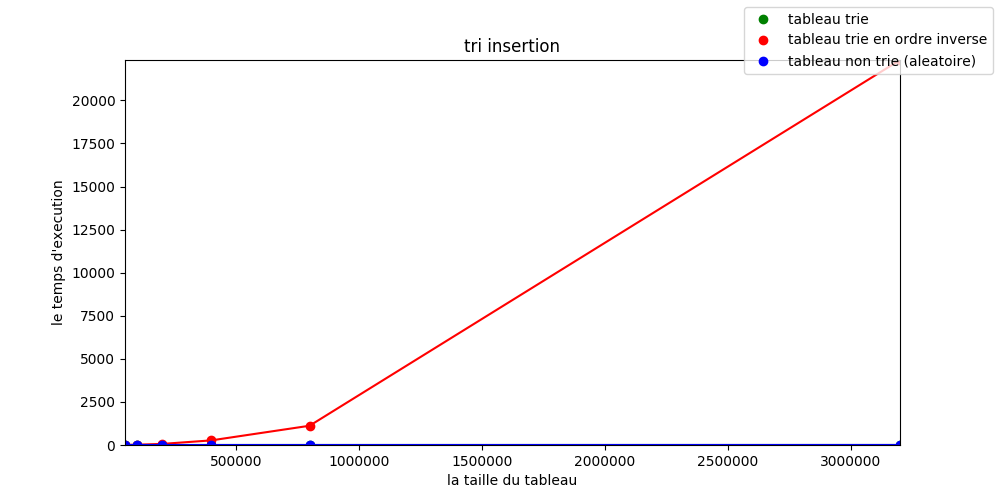
\includegraphics[width=1\textwidth]{graph/tri_insertion.png}

	
	\item Graphe des fonctions de la complexité théorique au Pire et Meilleur Cas.
	
	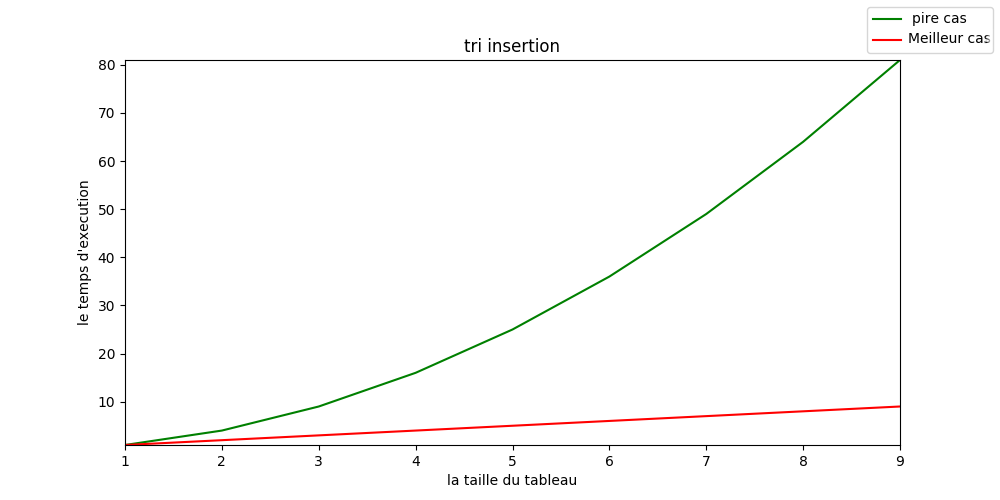
\includegraphics[width=1\textwidth]{graph/tri_insertion_teorique.png}

\end{enumerate}

\subsubsection{Comparaison de la complexité théorique avec la complexité expérimentale.}
On remarque que les temps d'exécution sont approximativement multiplies par 4 lorsque N est doublé pour: \color{blue} les tableaux en ordre inverse.\\
\color{black}

Exemples :\\
N1 = 100000 $\rightarrow$ T1 = 17.157000 \\
N2 = 200000 = 2 * N1 $\rightarrow$ T2 = 62.752000 $\approx$ 4 * T1 = 2² * T1\\

On en déduit que le temps d'exécution est proportionnel a N, ce que l'on peut représenter par la formule suivante :\\

\begin{center}

\color{red}
T1(x * N) = x² * T1(N) pour tous x * N qui appartient a [50000 - 2048000000]\\
\color{black}
(x etant la tangente d'un point sur le graphe).\\

\end{center}

 Puis l'on peut aussi constater que lorsque la taille N du \color{blue} tableau dans le bon ordre ou aléatoire \color{black} est doublé ,
 le temps d'exécution est lui aussi à peu près doublé.\\
 
 Exemples :\\
N1 = 50000 $\rightarrow$ T1 = 0.000225\\
N2 = 100000 = 2 * N1 $\rightarrow$ T2 = 0.000450 $\approx$ 2 * T1 \\

On en déduit que le temps d'exécution est proportionnel a N, ce que l'on peut représenter par la formule suivante :\\

\begin{center}

\color{red}
T2(x * N) = x * T2(N) pour tous x * N qui appartient a [50000 - 2048000000]\\
\color{black}
(x etant la tangente d'un point sur le graphe).\\

\end{center}

Ainsi nos données expérimentale de la complexité suivent une des deux fonctions T1 et T2. \\ 
Et la complexité théorique au pire cas est de l'ordre de : P(n) = $n^2$ \\
Et la complexité théorique au meilleur cas est de l'ordre de : M(n) = n \\

\begin{center}

On relève que :\\
\color{blue} 
 M(n) $\le$ T1(n) $\le$ P(n) tel que n $\le Cte^2$ * n $\le n^2$ \\
\color{black}
 avec Cte = 2 et n très grand\\
 
\end{center}

 et \\
 
\begin{center}

\color{blue} 
 M(n) $\le$ T2(n) $\le$ P(n) tel que n  $\le$ Cte * n $\le$ $n^2$ \\
\color{black}
 avec Cte = 2 et n très grand\\

\end{center}

 (les données obtenues par les testes sont majorées par les données du pire cas et minorées par les données au meilleur cas)\\
  
  On en conclue que :
\color{red}
 "Le modèle théorique est conforme avec les mesures expérimentales!"\\
\color{black}

\texttt{  }

\color{red}
Remarque:\\
\color{black}
Nous ne pouvant pas généraliser car les testes que nous avons fait n'englobent pas toutes les valeurs possibles.




\newpage




\subsection{Algorithme 2: Tri à bulles.}
\subsubsection{Description de la méthode de tri.}
Le tri à bulles consiste à parcourir un tableau à plusieurs reprises,
 en comparant les éléments du tableau deux à deux à chaque itération et en les permutant selon le tri (ascendant ou descendant).\\
 
Pour notre étude prenons le tri dans le cas ascendant.\\

Après un premier parcours du tableau, nous aurons l'élément le plus grand du tableau à la dernière position.\\

 Nous faisons la même chose une autre fois en excluant la dernière case du tableau  (qui à été triée au parcours précédent)
 et donc à la fin de ce nouveau parcours le nouvel élément le plus grand se retrouvera à l'avant dernière case du tableau.\\
  
 Nous faisons l'opération N-1 fois (en considérant N taille du tableau) et tel est le principe du tri à bulles.

\subsubsection{Écriture de l'algorithme.}
 Itératif
	\begin{sql}
procedure Tri_bulles(tab[]:d`entier,taille:entier)
	VAR
		i,j,n :entier;
	DEBUT
		Pour i de taille a 2 
		faire
			Pour j = 1 a i-1 
			faire
				SI (tab[j] > tab[j+1] ) 
				ALORS permuter(tab[j], tab[j+1]);
				FinSi;
			fait;
		fait;
	FIN.
	
procedure pérmuter(a:entier, b:entier)
	VAR
		temp :entier;
	DEBUT
		temp = a;
		a = b;
		b = temp;
	FIN.
	\end{sql}
	


\subsubsection{Calcule de la complexité Temporelle. }
Le tri à bulles est un algorithme de tri lent, on peut donc s'attendre à une complexité importante.

\begin{enumerate}
	\item Pire Cas
	(Il s'agit du cas où les éléments du tableau sont triés dans l'ordre inverse que celui souhaité)\\
	
	le programme effectue donc un nombre important de permutation, tel que sa complexité est de:\\
	\color{blue}
CT(n) = (n-2)+1 + ([n-1]-2)+1 +.....+1+0 = (n-1)+(n-2)+...+1 tests.\\

CT(n) =$\frac{N(N-1)}{2}$ tests.\\

	\color{black}

Soit en notation de Landau :
\color{blue}
 O(n²).\\
 
\color{black}

	
	\item Meilleur Cas
	(Il s'agit du cas où les éléments du tableau sont déjà triés.)\\
	
	 le programme effectue N² comparaison et aucune permutation,ainsi sa complexité est:\\
	 \color{blue}
	 CT(n) = N² tests.
	\color{black}

Soit en notation de Landau :
\color{blue}
 O(n²).
\color{black}

\end{enumerate}

\subsubsection{Calcule de la complexité Spatiale.}
Nous avons utiliser dans notre programme : un tableau de N éléments et 3 variables entières.\\
on considérant que la taille d'une entier est sur 4 Octets \\

nous obtenant :
\color{blue} CS(n) = 4(N + 3) Octets = 4N + 12 octets.
\color{black}
	
	Ainsi 
	\color{blue}
	CS(n) = O(n).
	\color{black}


\subsubsection{Écriture du programme en langage C.}
\begin{sql}
long long int *tri_bulles(long long int *tab,long long int size)
{
  long long int i,j,temp=0,n;
  n = size -1;
  for(i=n; i>=0; i--)
  {
    for(j=1;j<=i;j++)
    {
      if(tab[j] < tab[j-1])
      {
        temp = tab[j];
        tab[j] = tab[j-1];
        tab[j-1] = temp;
      }
    }
  }

  return tab;
}
\end{sql}

\subsubsection{Mesure des temps d'exécution.}
Grâce à l'exécution du programme C vu précédemment nous avons obtenu les temps d'exécution des trois (3) cas de tableaux.
\begin{enumerate}
	\item Données du tableau dans l'ordre.
	\item Données du tableau positionnées Aléatoirement.
	\item Données du tableau dans l'ordre inverse.
\end{enumerate}
\color{blue}
\textrm{  }
\\
\\
\begin{tabular}{|p{4cm}||p{1.8cm}|p{1.8cm}|p{1.8cm}|p{1.8cm}|p{1.8cm}|p{1.8cm}|}
\hline
Taille du Tableau (N) : & 50000 & 100000 & 200000 & 400000 & 800000  & 1600000\\
\hline
Temps (bon ordre) : & 6.344 & 25.352 & 101.355 & 415.429 & 1703.258 & 7153.687  \\
\hline

Temps (Aléatoire) : & 14.629 & 60.693 & 248.038 & 998.726 & 4125.610 & 16915.001\\
\hline

Temps (inverse) :  & 10.792 & 51.536 & 178.093 & 816.742 &  2751.297 & 11968.141  \\
\hline

\end{tabular}
\\
\\
\begin{tabular}{|p{4cm}||p{2.25cm}|p{2.25cm}|p{2.25cm}|p{2.25cm}|p{2.25cm}|}
\hline
Taille du Tableau (N) : & 3200000 & 6400000 & 12800000 & 25600000 &  51200000  \\
\hline

Temps (bon ordre) : &  30117.023 & 120468.095 & 503556.639 & 2125009.017 & 7798783.092   \\
\hline

Temps (Aléatoire) : & 69013.204 & 279503.476 & 1118013.906 & 4349074.095 & 17396696.380\\
\hline

Temps (inverse) : & 47872.567 & 189096.642 & 869844.556 & 3192329.524 & 12769318.100 \\
\hline

\end{tabular}
\color{black}

\subsubsection{Représentation Graphique.}
\begin{enumerate}
	\item Graphe des variation des temps d'exécution selon la taille N du tableau.

	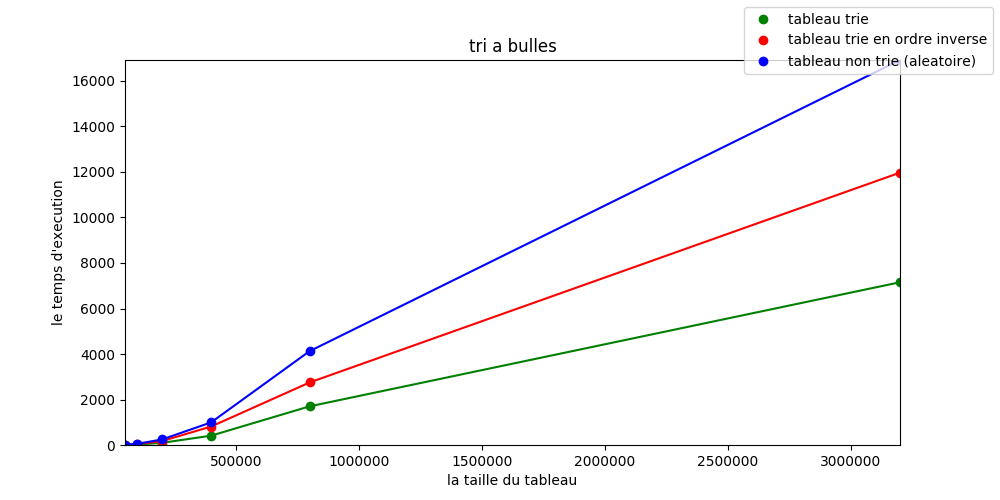
\includegraphics[width=1\textwidth]{graph/tri_bulles.png}
	
	
	\item Graphe des fonctions de la complexité théorique au Pire et Meilleur Cas.
	
	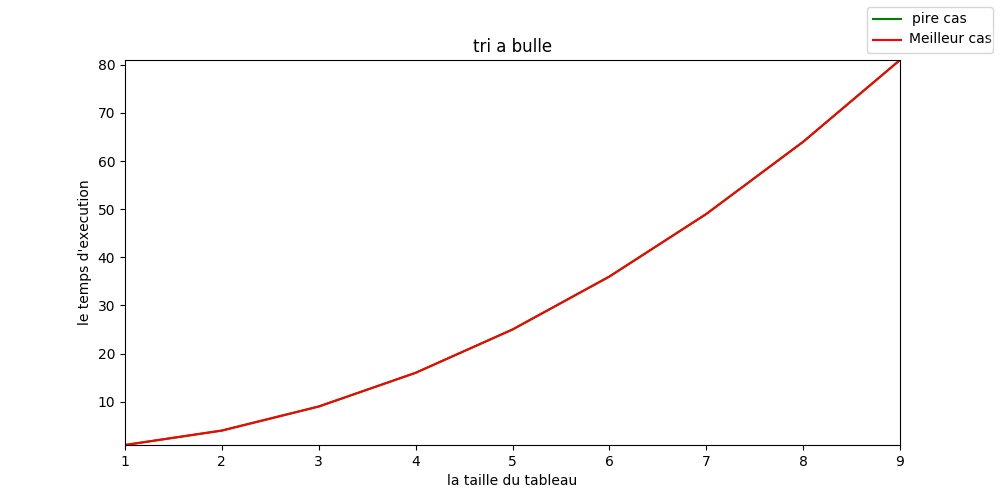
\includegraphics[width=1\textwidth]{graph/tri_bulle_teorique.png}
	
\end{enumerate}

\subsubsection{Comparaison de la complexité théorique avec la complexité expérimentale.}

  Nous remarquons que les temps d'exécution évoluent de manière quadratique, \\
  ce qui signifie que que si par exemple nous doublons le nombre de N en entrée, le temps d'exécution se voit multiplié par 4. \\

  Le temps d'exécution est donc proportionnel à N, et nous pouvons le représenter par la formule suivante : \\
 
\begin{center}

\color{red}
T(x * N) = x² * T(N) pour tous x * N qui appartient a [50000 - 2048000000]\\
\color{black}
(x etant la tangente d'un point sur le graphe).\\

\end{center}

  Exemple : \\
  N1 = 50000 => T1 = 14.629469\\
  N2 = 100000 = 2 * N1 $\rightarrow$ T2 = 60.693804 $\approx$ 4 * T1 = 2² * T1.\\

  NB : Quelque soit l'ordre des éléments du tableau \color{blue} (ordonnés, inverses ou aléatoire)\color{black},\\
  la complexité est toujours quadratique et la formule citée plus haut est toujours valide.\\

On relève que :
\begin{center}
\color{blue} 
 T(n) $\le$ P(n) tel que $ Cte^2$ * n $\le n^2$ \\
\color{black}
 avec Cte = 2 et n très grand\\
\end{center}

 (les données obtenues par les testes sont majorées par les données du pire cas)\\
  
  On en conclue que :
\color{red}
 "Le modèle théorique est conforme avec les mesures expérimentales!"\\
\color{black}

\texttt{  }

\color{red}
Remarque:\\
\color{black}
Nous ne pouvant pas généraliser car les testes que nous avons fait n'englobent pas toutes les valeurs possibles.




\newpage







\subsection{Algorithme 3: Tri fusion.}
\subsubsection{Description de la méthode de tri.}
    L'algorithme du tri par fusion suit fidèlement la méthodologie diviser-pour-régner. \\
    Dans cette méthode de tri, la liste non triée est divisée en N sous-listes, chacune ayant un élément (sachant qu'une liste d'un élément est considérée comme triée). \\
    Ensuite, il fusionne à plusieurs reprises ces sous-listes, pour obtenir des sous-listes triées, et à la fin on obtient une liste bien triée.\\
    
    La fusion est traitée comme suit:\\
        * Divisez la liste récursivement en deux moitiés jusqu'à ce qu'elle ne puisse plus être divisée.\\
        * Fusionner les listes plus petites dans la nouvelle liste dans l'ordre trié.\\
        
    NB : S'il n'y a qu'un seul élément dans la liste, il est déjà trié.
        

\subsubsection{Écriture de l'algorithme.}

 Récursif
 \begin{sql}
Procedure TriFusion( Liste[]:d`entier; debut, fin: entier)
	VAR
		i, j, milieu : entier
	DEBUT
		SI(debut >= fin) 
		ALORS
            DEBUT
                milieur = (debut + fin) div 2;
                TriFusion(Liste,debut,milieu);
                TriFusion(Liste,milieu+1,fin);
                Fusion(debut,milieu,milieu+1,fin);
        FinSi.
	FIN.

Procedure Fusion ( Liste[]:d`entier; debut1, fin1, debut2, fin2: entier )
	VAR
		i, j, k : entier
	DEBUT
		i = fisrt1;
		j = debut2;
		k = 0;
        Tantque (i<=fin1 et j<=fin2) 
        faire
			SI(Liste[i] < Liste[j]) 
			ALORS
				Debut  
					ListTmp[k] = Liste[i];
                    i = i+1;
                    k = k+1;
                fin;
			SINON
				Debut
                    ListTmp[k] = Liste[j];
                    j = j+1;
                    k = k+1;
                fin;
            FinSi;
		Fait;

		Tantque (i<=fin1) 
		Faire
			[k] = Liste[i]; i = i+1; k = k+1;
        Fait;

        Tantque (j<=fin2) 
        Faire
        	ListTmp[k] = Liste[j];
            j = j+1; k = k+1;
        Fait;
            
        Pour j = 0 a k 
        Faire
            Liste[first+j] = ListTmp[j];
        Fait;
	FIN.
 \end{sql}

\subsubsection{Calcule de la complexité Temporelle. }
 Au pire et meilleur cas il s'agit de la même complexité, tel que:
 CT(N) =
 \color{blue}
  \[ 
\left\{
\begin{array}{r c l}
2*CT(\frac{N}{2}) + 2*N \quad si	\quad	N \le 2\\
\!  1 \qquad sinon
\end{array}
\right.
\]
\color{black}
Pour les puissances de 2, on a  CT($2^{n}$) = 2 * CT($2^{n-1}$) + 2 *$ 2^n $\\

et on va montrer par récurrence sur n que\\
\color{blue}
 $CT(2^n) = n*2^{n+1}$\\
 
$ CT(2^n) = 2 * 2^n + 2 * CT(2^{n-1})\\
\texttt{  } \texttt{  } \texttt{  }\qquad = 2 * 2^n + 2 * (n-1) * 2^n\\
\texttt{  } \texttt{  } \texttt{  } \qquad = 2 * 2^n + (n-1) * 2^{n+1}\\
\texttt{  } \texttt{  } \texttt{  } \qquad = 2^{n+1} + (n-1) * 2^{n+1}\\
\texttt{  } \texttt{  } \texttt{  } \qquad = n * 2^{n+1}\\
 $
 \color{black}
 
 Par conséquent,$ CT(2^n) = log_{2}(2^n)*2^{n+1}$,\\
  et en majorant $CT(n) par CT(2^{log_{2}(n)})$ \\
  on obtient: $CT(n) = H((log_{2}(n)) * 2^{log_{2}(n)+1} = O(n * ln(n))$ 

Ainsi, nous avons une complexité au pire et au meilleur cas = 
\color{blue}
O(n * ln(n)).
\color{black}

\subsubsection{Calcule de la complexité Spatiale.}
L'algorithme de tri fusion n'utilise que le tableau de N éléments (à trier) ainsi que 6 variables entiers.\\

on considérant que la taille d'un entier est sur 4 Octets.
Nous obtenant la complexité spatiale :\\
\color{blue}
CS(N) = 4(N + 6) octets = 4N + 24 octets
\color{black}

Ainsi \color{blue}
CS(n) = O(N).
\color{black}

\subsubsection{Écriture du programme en langage C.}
\begin{sql}
#include <stdio.h>
#include <stdlib.h>
#include <time.h>
#include <math.h>

void merge(long long int tab[], long long int first1, long long int last1, long long int first2, long long int last2)
    {
        long long int i = first1;
        long long int j = first2;
        long long int k = 0;
        while (i<=last1 && j<=last2)
        {
            if (tab[i] < tab[j])
            {
                Tmp[k] = tab[i];
                i++;
                k++;
            }
            else
            {
                Tmp[k] = tab[j];
                k++;
                j++;
            }
        }
        while (i<=last1) 
        {
            Tmp[k] = tab[i];
            k++;
            i++;
        }
        while (j<=last2)
        {
            Tmp[k] = tab[j];
            k++;
            j++;
        }
        for (j=0; j<k; j++)
            tab[first1+j] = Tmp[j];
    }


void MergeSort(long long int tab[] , long long int first, long long int last)
    {
        long long int middle,i,j;
        if (first>=last) return;
        middle = (first+last)/2;
        MergeSort(tab,first,middle);
        MergeSort(tab,middle+1,last);
        merge(tab,first,middle,middle+1,last);
    }
\end{sql}

\subsubsection{Mesure des temps d'exécution.}
\begin{enumerate}
	\item Données du tableau dans l'ordre.
	\item Données du tableau positionnées Aléatoirement.
	\item Données du tableau dans l'ordre inverse.
\end{enumerate}
Grâce à l'exécution du programme C vu précédemment nous avons obtenu les temps d'exécution des trois (3) cas de tableaux.

\color{blue}
\textrm{  }
\\
\\
\begin{tabular}{|p{4cm}||p{1.8cm}|p{1.8cm}|p{1.8cm}|p{1.8cm}|p{1.8cm}|p{1.8cm}|}
\hline
Taille du Tableau (N) : & 50000 & 100000 & 200000 & 400000 & 800000  & 1600000\\
\hline
Temps (bon ordre) : & 0.010 & 0.020 &  0.042 & 0.088 &  0.190 & 0.492 \\
\hline

Temps (Aléatoire) : & 
0.029 &  0.043 & 0.072 &  0.129 & 0.270 & 0.578 \\
\hline

Temps (inverse) :  & 0.009 & 0.019 & 0.040 & 0.101 & 0.203 & 0.368 \\
\hline

\end{tabular}
\\
\\
\begin{tabular}{|p{4cm}||p{2.25cm}|p{2.25cm}|p{2.25cm}|p{2.25cm}|p{2.25cm}|}
\hline
Taille du Tableau (N) : & 3200000 & 6400000 & 12800000 & 25600000 &  51200000  \\
\hline

Temps (bon ordre) : &   1.379 & 2.682 & 4.067 &  7.016 & 13.812   \\
\hline

Temps (Aléatoire) : & 
1.169 & 2.415 & 5.593 & 11.062 & 27.367  \\
\hline

Temps (inverse) : & 0.839 & 1.595 & 3.502 & 7.014 & 15.584 \\
\hline

\end{tabular}
\color{black}

\subsubsection{Représentation Graphique.}
\begin{enumerate}
	\item Graphe des variation des temps d'exécution selon la taille N du tableau.
	
	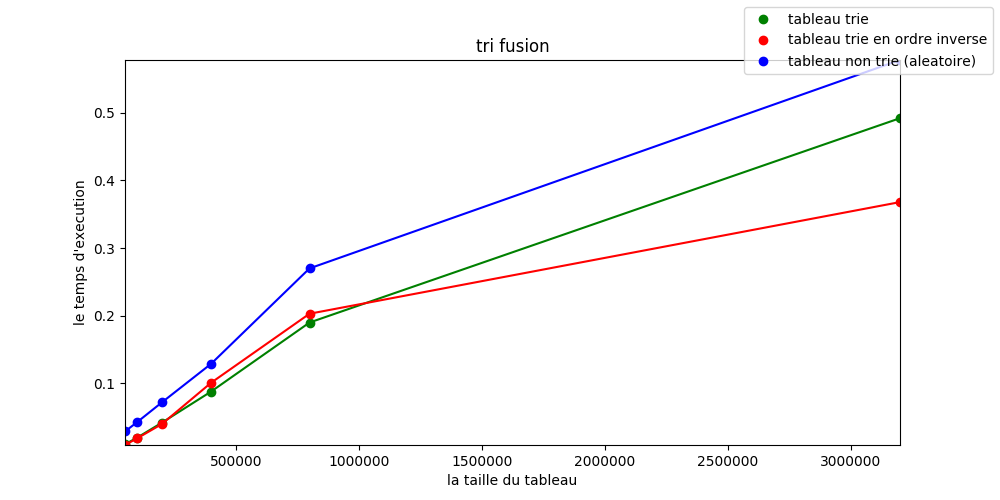
\includegraphics[width=1\textwidth]{graph/tri_fusion.png}
	
	
	\item Graphe des fonctions de la complexité théorique au Pire et Meilleur Cas.

	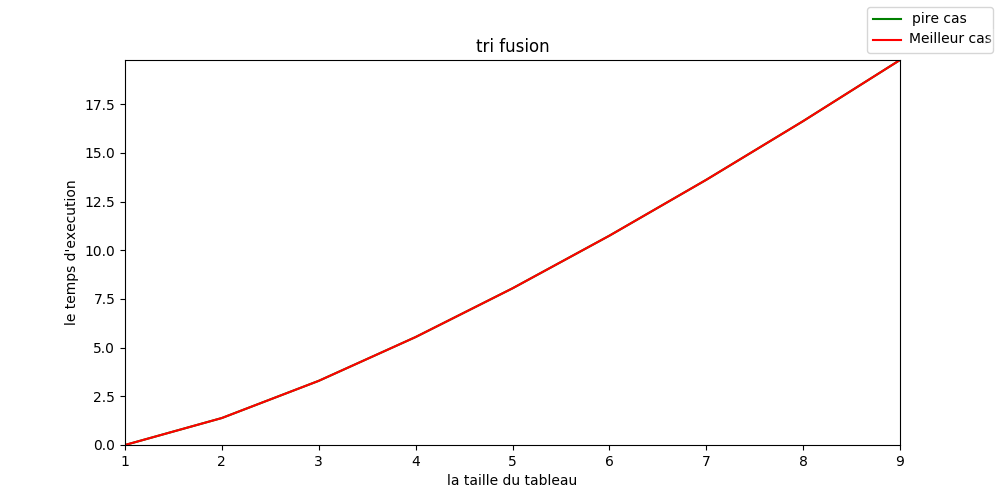
\includegraphics[width=1\textwidth]{graph/tri_fusion_teorique.png}	
	
\end{enumerate}

\subsubsection{Comparaison de la complexité théorique avec la complexité expérimentale.}

 On remarque que les temps d'exécution sont approximativement multiplies par 2 lorsque N est doublé pour: \color{blue} les tableaux en ordre croissant, en ordre inverse et même en ordre aléatoire.\\
\color{black}

Exemples :\\
N1 = 50000 $\rightarrow$ T1 = 0.010 \\
N2 = 100000 = 2 * N1 $\rightarrow$ T2 = 0.020 $\approx$ 2 * T1\\

On en déduit que le temps d'exécution est proportionnel a N, ce que l'on peut représenter par la formule suivante :\\

\begin{center}

\color{red}
T1(x * N) = x * T1(N) pour tous x * N qui appartient a [50000 - 2048000000]\\
\color{black}
(x etant la tangente d'un point sur le graphe).\\

\end{center}

Ainsi nos données expérimentale de la complexité suivent la fonctions T1. \\ 
Et la complexité théorique au pire et au meilleur cas est de l'ordre de : M(n) = n * log(n)\\

\begin{center}

  On en conclue que :
\color{red}
 "Le modèle théorique est conforme avec les mesures expérimentales!"\\
\color{black}
\end{center}
\texttt{  }

\newpage



\subsection{Algorithme 4: Tri rapide.}
\subsubsection{Description de la méthode de tri.}
 Cette méthode illustre le principe dit « diviser pour régner »
 
Le principe du Tri Rapide est de parcourir le tableau Tab = (t1, t2, ... , tn) en le divisant systématiquement en deux sous-tableaux Tab1 et Tab2.
 L'un est tel que tous ses éléments sont inférieurs à tous ceux de l'autre tableau et en travaillant séparément sur chacun des deux sous-tableaux
 en ré-appliquant la même division à chacun des deux sous-tableaux jusqu'à obtenir uniquement des sous-tableaux à un seul élément.

 C'est un algorithme dichotomique qui divise donc le problème en deux sous-problèmes dont les résultats sont réutilisés par re-combinaison,

Pour partitionner un tableau Tab en deux sous-tableaux Tab1 et Tab2 :
◦On choisit une valeur quelconque dans le Tableau appelée pivot (dans se qui va suivre se sra le 1er élément,
◦Le sous-tableau Tab1 va contenir tous les éléments de Tab inférieure ou égale au pivot,
◦Et le sous-tableau Tab2 tous les éléments de Tab supérieure au pivot.

- Ainsi de proche en proche en subdivisant le problème en deux sous-problèmes, à chaque étape, nous obtenons un pivot bien placé.

- Une procédure QuickSort va réaliser cette action .Cette procédure est récursive puisqu'on la ré-applique sur les deux sous-tableaux obtenues.
 
\subsubsection{Écriture de l'algorithme.}
\begin{enumerate}
	\item Itératif
	\begin{sql}
procedure permuter( a* :entier, b* :entier)
	VAR
		temp: entier;
	DEBUT
		temp = *a;
		*a = *b;
		*b = temp;
	FIN.

	fonction Partition(data[1..n]:entier, left:entier, right:entier):entier
	VAR
		x,i,j:entier;
	
	DEBUT
		x = data[right];
		i = (left - 1);
		
		POUR j de left a j right - 1 pas 1)
		FAIRE
			SI(data[j] <= x)
				ALORS
					++i;
					permuter(&data[i], &data[j]);
			FIN SI;
		FAIT;
			permuter(&data[i + 1], &data[right]);
			return (i + 1);
	FIN.

	Procadure QuickSortIterative( data[1..n]:entier, count:entier) 
	VAR
		startIndex,endIndex,top:entier;
		stack* :entier;
	
	DEBUT
		startIndex = 0;
		endIndex = count - 1;
		top = -1;
		stack = (entier*)Allouer(Taille(entier) * count);
		stack[++top] = startIndex;
		stack[++top] = endIndex;
		TANT QUE(top >= 0)
			FAIRE
				endIndex = stack[top--];
				startIndex = stack[top--];

				p:entier;
				p = Partition(data, startIndex, endIndex);

				SI(p - 1 > startIndex)
				ALORS
					DEBUT
						stack[++top] = startIndex;
						stack[++top] = p - 1;
					FIN;
				FIN SI;

				SI(p + 1 < endIndex)
				ALORS
					DEBUT
						stack[++top] = p + 1;
						stack[++top] = endIndex;
					FIN
				FIN SI;			
			FAIT;
			Libérer(stack);
		FIN.
	\end{sql}
	
\newpage	
	
	\item Récursif
	\begin{sql}			
	procedure pérmuter(tableau[] :entier,a:entier, b:entier)
		VAR
			temp :entier;	
		DEBUT
			temp = tableau[a];
			tableau[a] = tableau[b];
			tableau[b] = temp;
		FIN
				
	/*********************************************************/

	procedure quickSort(tableau[]:entier,debut:entier, fin:entier)
	VAR
		gauche, droit :entier;
		pivot :entier;
					
	DEBUT
		gauche = debut-1;
		droite = fin+1;
		CONST pivot = tableau[debut];

		/* Si le tableau est de longueur nulle, il n'y a rien a faire. */
		SI(debut >= fin)
			ALORS return;
		FIN SI;
		/* Sinon, on parcourt le tableau, une fois de droite a gauche, et une
	   autre de gauche a droite, a la recherche d'éléments mal placés,
	   que l'on permute. Si les deux parcours se croisent, on arrete. */
	
		TANT QUE(1)
		FAIRE
			REPETER 
			droite = droit - 1; 
			JUSQU`A(tableau[droite] > pivot);
							
			REPETER
			gauche = gauche + 1; 
			JUSQU`A(tableau[gauche] < pivot);

			SI(gauche < droite)
				ALORS pérmuter(tableau, gauche, droite);
				SINON break;
			FIN SI;
		FAIT;

		/* Maintenant, tous les éléments inférieurs au pivot sont avant ceux
	   supérieurs au pivot. On a donc deux groupes de cases a trier. On utilise
	   pour cela... la méthode quickSort elle-meme ! */
					   
		quickSort(tableau, debut, droite);
		quickSort(tableau, droite+1, fin);
	FIN.
	\end{sql}
\end{enumerate}

\subsubsection{Calcule de la complexité Temporelle. }
\begin{enumerate}
	\item Pire Cas
	(il s'agit d'un tableau trié dans l'ordre inverse avec choix du 1er élément comme pivot )\\
	
		le 1er élément (plus grand) du tableau sera pris en pivot tous le tableau sera parcouru pour atteindre de n ième élément (plus petit) afin de les permuter puis,\\
		
		ainsi le n ième élément (plus grand) sera à sa place, on vérifie pour le 1er élément (plus petit) qui s'avère aussi a sa place donc pas de permutation 
		(mais tous le tableau est parcouru pour s'en rendre compte).
		On se retrouve dans la situation : le n-1 ième élément(2eme plus grande valeur du tableau), a été permutée avec le 2eme,\\
		
		puis, comme toutes les autres valeurs sont inférieures au n-1 ième élément, nos deux recherches d'éléments mal placés se sont « croisées »,
		et on n'a rien permuté de plus.\\
		
	De même, après cette étape, un autre passage déterminera que le 2eme est bien placé et qu'on peut l'ignorer après avoir comme même parcouru tous le tableau.\\
	
	Ce schéma se répètera ainsi jusqu'à ce que tout le tableau soit trié. On se rend compte que, à chaque étape,\\
	
	on place correctement une valeur et que, pour ce faire, on parcourt tout l'ensemble tableau à trier. \\
	
	
	Ainsi, le premier passage fait n tests, le second n-1, et ainsi de suite. Au final, on aura effectué \color{blue}  N + (N - 1) + (N - 2) + ... + 3 + 2 + 1 tests,\color{black}\\
	 
	et N permutations. En calculant la somme \color{blue} N + (N - 1) + (N - 2) + ... + 3 + 2 + 1, \color{black}\\
	 on trouve qu'elle est égale à \color{blue} $\frac{N*(N+1)}{2} = \frac{N^2}{2} + \frac{N}{2}$\\
	\color{black}
	
	soit en notation landau
	\color{blue} O(N²).
	\color{black}\\
	\texttt{  }\\
	
	
	\item Meilleur Cas
	(il s'agit des tableaux dont le pivot est proche de la médiane de ces derniers)\\
	
	Nous devons d'abord remarquer qu'à chaque étape du processus, nous doublons le nombre de sous-tableaux considérés, 
	mais que la taille de chacun de ces sous-tableaux est divisée par deux. Donc, au final, chaque étape demandera N opérations.\\
	

	Il nous faut maintenant compter le nombre d'étapes nécessaires pour trier un tableau.
	Pour cela, Le tri est bien évidemment terminé lorsque nous atteignons des sous-tableaux de taille 1. \\
	
	Donc : il y a autant d'étapes que de divisions par 2 nécessaires pour passer de N à 1. 
	La fonction qui nous donne \color{blue} « combien de fois diviser N par 2 avant d'arriver à 1 » \color{black} est la fonction logarithme de base 2 : \color{blue} "$Log_{2}$". \color{black} \\
	

	Du coup, le tri rapide a un complexité au cas moyen:\color{blue} O(N * $log_{2}$(N)). \color{black}
\end{enumerate}

\subsubsection{Calcule de la complexité Spatiale.}
Nous avons 1 tableau d'entier à N éléments ainsi que 3 variables entières \\

	on considérant que la taille d'un entier est sur 4 Octets, 
	nous obtenant : \color{blue} CS(n) = 4(N + 3) Octets = 4N + 12 octets.\color{black}
	
	Ainsi \color{blue} CS(n) = O(n). \color{black}



\subsubsection{Écriture du programme en langage C.}
\begin{sql}
#include<stdio.h>
#include<stdlib.h>
#include<time.h>
		
	void pérmuter(int tableau[], int a, int b)
	{
		int temp = tableau[a];
		tableau[a] = tableau[b];
		tableau[b] = temp;
	}
				
	/***************************************************************/

	void quickSort(int tableau[], int debut, int fin)
	{
		int gauche = debut-1;
		int droite = fin+1;
		const int pivot = tableau[debut];

		if(debut >= fin)
		return;

		while(1)
		{
			do droite--; while(tableau[droite] > pivot);
			do gauche++; while(tableau[gauche] < pivot);

			if(gauche < droite)
				pérmuter(tableau, gauche, droite);
				else break;
		}

		quickSort(tableau, debut, droite);
		quickSort(tableau, droite+1, fin);
	}
\end{sql}

\subsubsection{Mesure des temps d'exécution.}

Grâce à l'exécution du programme C vu précédemment nous avons obtenu les temps d'exécution des trois (3) cas de tableaux.
\begin{enumerate}
	\item Données du tableau dans le bon ordre.
	\item Données du tableau positionnées Aléatoirement.
	\item Données du tableau dans l'ordre inverse.
\end{enumerate}
\color{blue}
\textrm{  }
\\
\begin{tabular}{|p{4cm}||p{1.8cm}|p{1.8cm}|p{1.8cm}|p{1.8cm}|p{1.8cm}|p{1.8cm}|}
\hline
Taille du Tableau (N) : & 50000 & 100000 & 200000 & 400000 & 800000  & 1600000\\
\hline
Temps (bon ordre) : & 15.067 & 59.997 & 243.606 & 962.812 & 3864.314 & 15379.962 \\
\hline

Temps (Aléatoire) : & 0.015 & 0.033 & 0.062 & 0.132 & 0.325 & 2.700 \\
\hline

Temps (inverse) :  & 9.787 & 38.979 & 157.157 & 627.971 & 2527.851 & 10451.672  \\
\hline

\end{tabular}
\\
\begin{tabular}{|p{4cm}||p{2.25cm}|p{2.25cm}|p{2.25cm}|p{2.25cm}|p{2.25cm}|}
\hline
Taille du Tableau (N) : & 3200000 & 6400000 & 12800000 & 25600000 &  51200000  \\
\hline

Temps (bon ordre) : &  61519.878 & 243618.724 & 979347.255 & 3917389.023 & 15638216.980   \\
\hline

Temps (Aléatoire) : & 9.100 & 32.848 & 124.024 & 458.888 & 1762.132  \\
\hline

Temps (inverse) : & 43897.022 & 182172.643 & 769679.415 & 3087953.419 & 12870591.520  \\
\hline

\end{tabular}
\color{black}

\subsubsection{Représentation Graphique.}
\begin{enumerate}
	\item Graphe des variation des temps d'exécution selon la taille N du tableau.

	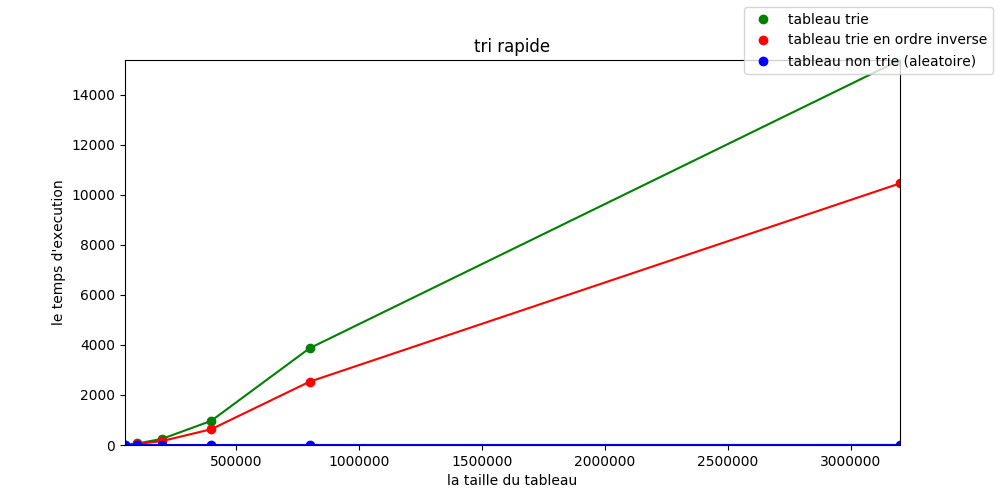
\includegraphics[width=1\textwidth]{graph/tri_rapide.png}
	
	
	\item Graphe des fonctions de la complexité théorique au Pire et Meilleur Cas.
	
	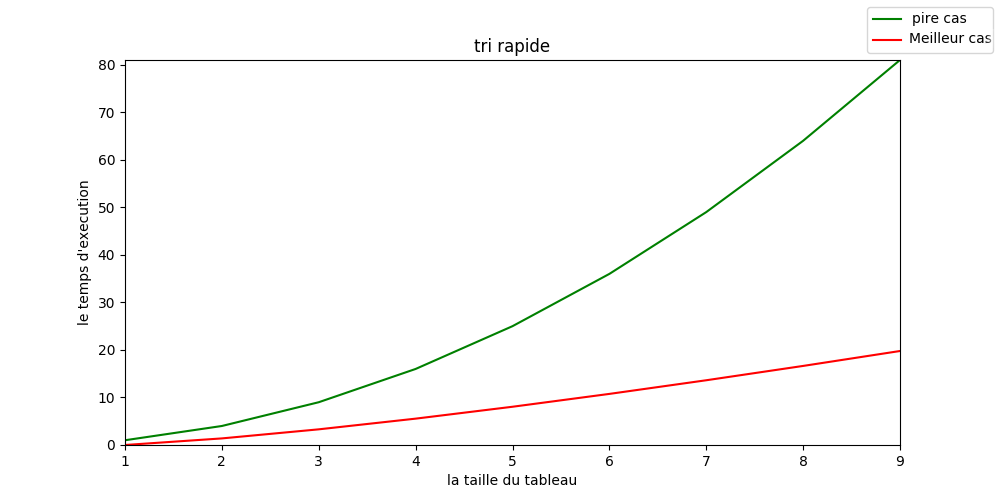
\includegraphics[width=1\textwidth]{graph/tri_rapide_teorique.png}
	
\end{enumerate}

\subsubsection{Comparaison de la complexité théorique avec la complexité expérimentale.}

 On remarque que les temps d'exécution sont approximativement multiplies par 4 lorsque N est doublé pour: \color{blue} les tableaux en ordre croissant et en ordre inverse.\\
\color{black}

Exemples :\\
N1 = 50000 $\rightarrow$ T1 = 9.787000 \\
N2 = 100000 = 2 * N1 $\rightarrow$ T2 = 38.979000 $\approx$ 4 * T1 = 2² * T1\\

Aussi\\
N1 = 400000 $\rightarrow$ T1 = 627.971000\\
N2 = 800000 = 2 * N1 $\rightarrow$ T2 = 2527.851000 $\approx$ 4 * T1 = 2² * T1\\

On en déduit que le temps d'exécution est proportionnel a N, ce que l'on peut représenter par la formule suivante :\\

\begin{center}

\color{red}
T1(x * N) = x² * T1(N) pour tous x * N qui appartient a [50000 - 2048000000]\\
\color{black}
(x etant la tangente d'un point sur le graphe).\\

\end{center}

 Puis l'on peut aussi constater que lorsque la taille N du \color{blue} tableau en ordre aléatoire \color{black} est doublé ,
 le temps d'exécution est lui aussi à peu près doublé.\\
 
 Exemples :\\
N1 = 50000 $\rightarrow$ T1 = 0.015000\\
N2 = 100000 = 2 * N1 $\rightarrow$ T2 = 0.033000 $\approx$ 2 * T1 \\

Aussi\\
N1 = 400000 $\rightarrow$ T1 = 0.132000 \\
N2 = 800000 = 2 * N1 $\rightarrow$ T2 =  0.325000 $\approx$ 2 * T1 \\

On en déduit que le temps d'exécution est proportionnel a N, ce que l'on peut représenter par la formule suivante :\\

\begin{center}

\color{red}
T2(x * N) = x * T2(N) pour tous x * N qui appartient a [50000 - 2048000000]\\
\color{black}
(x etant la tangente d'un point sur le graphe).\\

\end{center}

Ainsi nos données expérimentale de la complexité suivent une des deux fonctions T1 et T2. \\ 
Et la complexité théorique au pire cas est de l'ordre de : P(n) = $n^2$ \\
Et la complexité théorique au meilleur cas est de l'ordre de : M(n) = n * log(n)\\

\begin{center}

On relève que :\\
\color{blue} 
 M(n) $\le$ T1(n) $\le$ P(n) tel que n * log(n) $\le Cte^2$ * n $\le n^2$ \\
\color{black}
 avec Cte = 2 et n très grand\\
 
\end{center}

 et \\
 
\begin{center}

\color{blue} 
 M(n) $\le$ T2(n) $\le$ P(n) tel que n * log(n) $\le$ Cte * n $\le$ $n^2$ \\
\color{black}
 avec Cte = 2 et n très grand\\

\end{center}

 (les données obtenues par les testes sont majorées par les données du pire cas et minorées par les données au meilleur cas)\\
  
  On en conclue que :
\color{red}
 "Le modèle théorique est conforme avec les mesures expérimentales!"\\
\color{black}

\texttt{  }

\color{red}
Remarque:\\
\color{black}
Nous ne pouvant pas généraliser car les testes que nous avons fait n'englobent pas toutes les valeurs possibles.



\newpage




\subsection{Algorithme 5: Tri par tas.}
\subsubsection{Description de la méthode de tri.}
Cet algorithme consiste à voir le tableau comme un arbre binaire. 
Le premier élément est la racine, ces deux descendants sont les éléments 2n et 2n+1 
(nous suivons ce même principe pour tous les éléments du tableau).\\

Dans l'algorithme, on cherche à obtenir un tas, c'est-à-dire un arbre binaire vérifiant les propriétés suivantes: 

la différence maximale de profondeur entre deux feuilles est de 1 
(i.e. toutes les feuilles se trouvent sur la dernière ou sur l'avant-dernière ligne) ;
les feuilles de profondeur maximale sont « tassées » sur la gauche.\\
chaque nœud est de valeur supérieure (resp. inférieure) à celles de ses deux fils, 
pour un tri ascendant (resp. descendant).\\
Il en découle que la racine du tas (le premier élément) contient la valeur maximale (resp. minimale) de l'arbre. 
Le tri est fondé sur cette propriété.

L'opération de base de ce tri est le tamisage d'un élément.
 Cette opération consiste à échanger la racine avec le plus grand de ses fils,
 et ainsi de suite récursivement jusqu'à ce qu'elle soit à sa place. \\
 La racine de ce tas est donc la valeur maximale du tableau.
 Puis on échange la racine avec le dernier élément du tableau, 
 et on restreint le tas en ne touchant plus au dernier élément, 
 c'est-à-dire à l'ancienne racine ;\\
 on a donc ainsi placer la valeur la plus haute en fin de tableau (donc à sa place), 
 et l'on n'y touche plus. Puis on tamise la racine pour créer de nouveau un tas,
 et on répète l'opération sur le tas restreint jusqu'à l'avoir vidé et remplacé par un tableau trié.\\ 

\subsubsection{Écriture de l'algorithme.}
 Itératif
 \begin{sql}
Procedure tri_tas(arbre[]:d`entier, longueur:entier)
VAR
	i : entier;
DEBUT
   Pour i := longueur/2 a 1
       tamiser(arbre, i, longueur);
   Fait;
   Pour i := longueur a 2
       permuter(arbre[1],arbre[i]);
       tamiser(arbre, 1, i-1);
   Fait;
FIN.

Procedure tamiser(arbre, noeud, n)
VAR
	k := noeud
	j := 2*k
DEBUT
	Tant que j <= n
	    SI (j < n et arbre[j] < arbre[j+1])
    	ALORS j := j+1;
    	FinSi;
    
    	SI (arbre[k] < arbre[j])
    	ALORS
    		permuter(arbre[k],arbre[j]);
    	    k := j;
    	    j := 2*k;
		SINON
			j := n+1
    	FinSi;
	Fait;
FIN.
 \end{sql}


\subsubsection{Calcule de la complexité Temporelle. }
Au pire et Meilleur cas il s'agit de la même complexité, tel que\\

Dans cet algorithme nous faisons appel à la fonction tamiser: \color{blue} n fois.\color{black}\\
 et à l'intérieur de la fonction tamiser le parcours du tableau (qui est à présent sous forme d'un arbre), se fait deux éléments à la fois, puis pour chaque élément aussi 2 fils, ...ect\\
se qui donne une complexité de l'ordre de :\color{blue} log(n).\color{black}
Ainsi nous obtenant un complexité asymptotique de Landau :\\
\color{blue}
CT(n) = O(n log n);\\
\color{black}

Le nombre d'échanges dans le tas est majoré par le nombre de comparaisons et il est du même ordre de grandeur.\\
La complexité au pire en nombre de transferts du tri par tas est donc en \color{blue} O(n log n). \color{black}



\subsubsection{Calcule de la complexité Spatiale.}
Dans le programme principale nous avons :\\
-Le tableau de taille N.\\
-Sa longueur n qui est un entier.\\
-Une variable i entière.\\

Dans la fonction tamiser nous avons : \\
-Notre tableau de taille N\\
-Un noeud qui est un entier.\\
-la taille du tableau qui est un entier.\\
-Deux variables de type entier j et k.\\

	on considérant que la taille d'un entier est sur 4 Octets, 
	nous obtenant : \color{blue} CS(n) = 4(2N + 6) Octets = 8N + 24 octets.\color{black}
	
	Ainsi \color{blue} CS(n) = O(n). \color{black}



\subsubsection{Écriture du programme en langage C.}
\begin{sql}
void makeheap ( long long int x[ ], long long int n )
{
   long long  int i, val, s, f ;
    for ( i = 1 ; i < n ; i++ )
    {
        val = x[i] ;
        s = i ;
        f = ( s - 1 ) / 2 ;
        while ( s > 0 && x[f] < val )
        {
            x[s] = x[f] ;
            s = f ;
            f = ( s - 1 ) / 2 ;
        }
        x[s] = val ;
    }
}

void heapsort ( long long int x[ ], long long int n )
{
    long long int i, s, f, ivalue ;
    for ( i = n - 1 ; i > 0 ; i-- )
    {
        ivalue = x[i] ;
        x[i] = x[0] ;
        f = 0 ;

        if ( i == 1 ) s = -1 ;
        else s = 1 ;

        if ( i > 2 && x[2] > x[1] )  s = 2 ;

        while ( s >= 0 && ivalue < x[s] )
        {
            x[f] = x[s] ;
            f = s ;
            s = 2 * f + 1 ;

            if ( s + 1 <= i - 1 && x[s] < x[s + 1] ) s++ ;
            if ( s > i - 1 )  s = -1 ;
        }
        x[f] = ivalue ;
    }
}
\end{sql}

\subsubsection{Mesure des temps d'exécution.}
\begin{enumerate}
	\item Données du tableau dans l'ordre.
	\item Données du tableau positionnées Aléatoirement.
	\item Données du tableau dans l'ordre inverse.
\end{enumerate}
Grâce à l'exécution du programme C vu précédemment nous avons obtenu les temps d'exécution des trois (3) cas de tableaux.

\color{blue}
\textrm{  }
\\
\begin{tabular}{|p{4cm}||p{1.8cm}|p{1.8cm}|p{1.8cm}|p{1.8cm}|p{1.8cm}|p{1.8cm}|}
\hline
Taille du Tableau (N) : & 50000 & 100000 & 200000 & 400000 & 800000  & 1600000\\
\hline
Temps (bon ordre) : & 0.000515 & 0.001030 & 0.002083 & 0.004566 & 0.008513 & 0.165864  \\
\hline

Temps (Aléatoire) : & 0.008536 & 0.011043 & 0.021991 & 0.045623 & 0.045623 & 0.092964 \\
\hline

Temps (inverse) :  & 0.013019 & 0.030760 & 0.056678 & 0.117674 & 0.251907 & 5.836609  \\
\hline

\end{tabular}
\\
\begin{tabular}{|p{4cm}||p{2.25cm}|p{2.25cm}|p{2.25cm}|p{2.25cm}|p{2.25cm}|}
\hline
Taille du Tableau (N) : & 3200000 & 6400000 & 12800000 & 25600000 &  51200000  \\
\hline

Temps (bon ordre) : & 0.331613 & 0.663114 & 1.326228 & 2.387210 & 3.819536   \\
\hline

Temps (Aléatoire) : & 2.399831 & 5.342937 & 11.343149 & 23.820619 & 47.164813 \\
\hline

Temps (inverse) :  & 12.060041 & 25.115368 & 51.001254 & 98.978215 & 205.365220  \\
\hline

\end{tabular}
\color{black}

\subsubsection{Représentation Graphique.}
\begin{enumerate}
	\item Graphe des variation des temps d'exécution selon la taille N du tableau.
	
	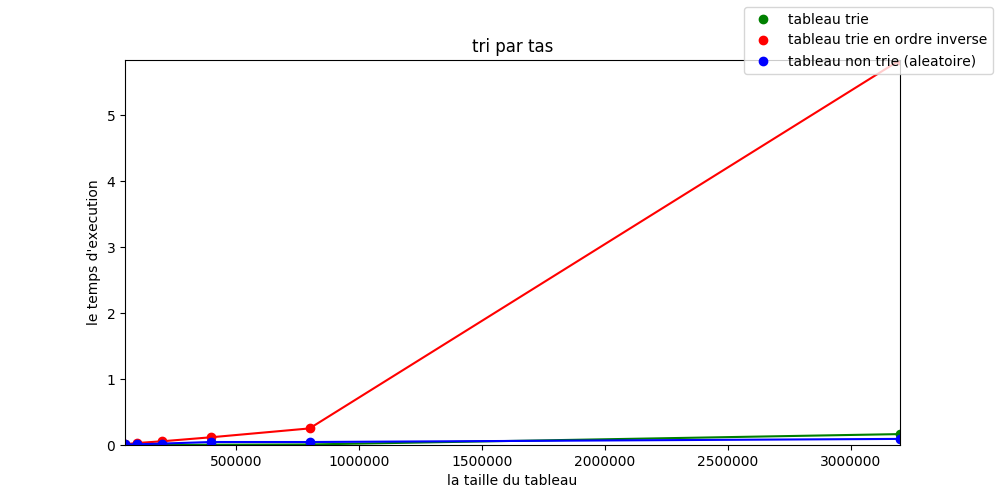
\includegraphics[width=1\textwidth]{graph/tri_tas.png}
	
	
	\item Graphe des fonctions de la complexité théorique au Pire et Meilleur Cas.
	
	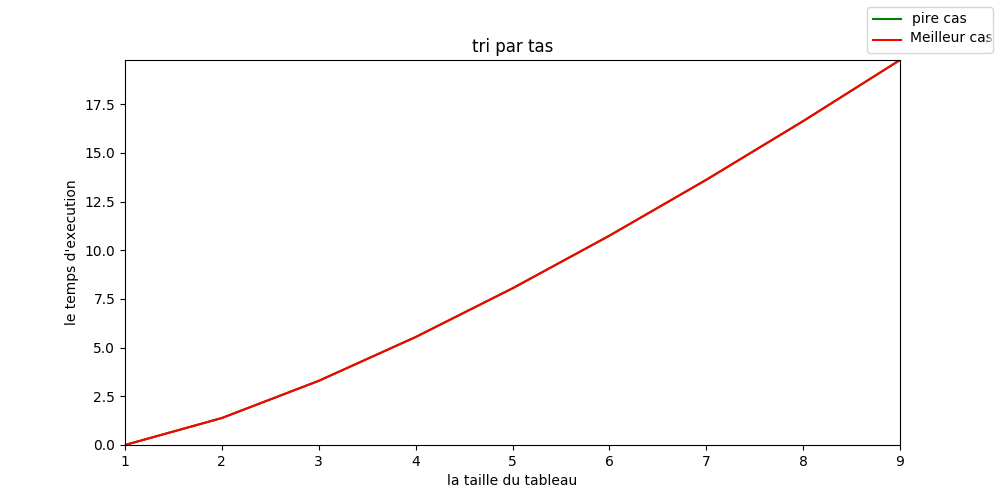
\includegraphics[width=1\textwidth]{graph/tri_tas_teorique.png}
	
\end{enumerate}

\subsubsection{Comparaison de la complexité théorique avec la complexité expérimentale.}


 Nous remarquons que les temps d'exécution évoluent de manière logarithmique, \\
  ce qui signifie que que si par exemple nous doublons le nombre de N en entrée, le temps d'exécution se voit aussi doublé. \\

  Le temps d'exécution est donc proportionnel à N, et nous pouvons le représenter par la formule suivante : \\
 
\begin{center}

\color{red}
T(x * N) = x * T(N) pour tous x * N qui appartient a [50000 - 2048000000]\\
\color{black}
(x etant la tangente d'un point sur le graphe).\\

\end{center}

  Exemple : \\
  N1 = 50000 $\rightarrow$ T1 = 0.00515
  N2 = 100000 = 2 * N1 $\rightarrow$ T2 = 0.001030 $\approx$ 2 * T1.\\

  NB : Quelque soit l'ordre des éléments du tableau \color{blue} (ordonnés, inverses ou aléatoire)\color{black},\\
  la complexité est toujours quadratique et la formule citée plus haut est toujours valide.\\

On relève que :
\begin{center}
\color{blue} 
 T(n) $\approx$ P(n) tel que Cte * n $\approx$ n*log(n) \\
\color{black}
 avec Cte = 2 et n très grand\\
\end{center}

 (les données obtenues par les testes sont proche des données de la complexité théorique)\\
  
  On en conclue que :
\color{red}
 "Le modèle théorique est conforme avec les mesures expérimentales!"\\
\color{black}

\texttt{  }

\color{red}
Remarque:\\
\color{black}
Nous ne pouvant pas généraliser car les testes que nous avons fait n'englobent pas toutes les valeurs possibles.




\newpage


\section{Partie II: Comparaison des Algorithmes.}
\subsection{Représentation des graphes des complexités des cinq (5) algorithmes.}
\subsubsection{Complexité théorique.}

1. Comparaison de la Complexité théorique au pire cas pour les cinq (5) algorithmes
	
		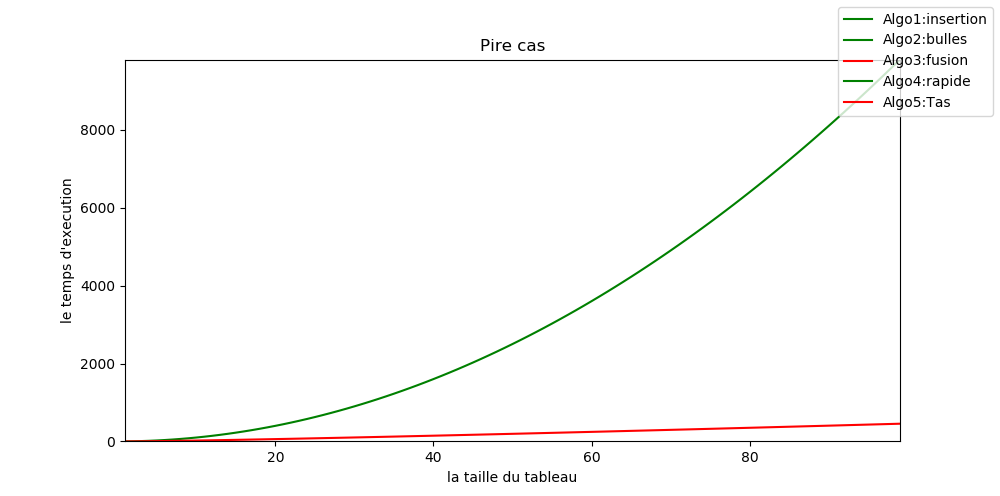
\includegraphics[width=1\textwidth]{graph/All_pire.png}
	
	
2. Comparaison de la Complexité théorique au meilleur cas pour les cinq (5) algorithmes
		
			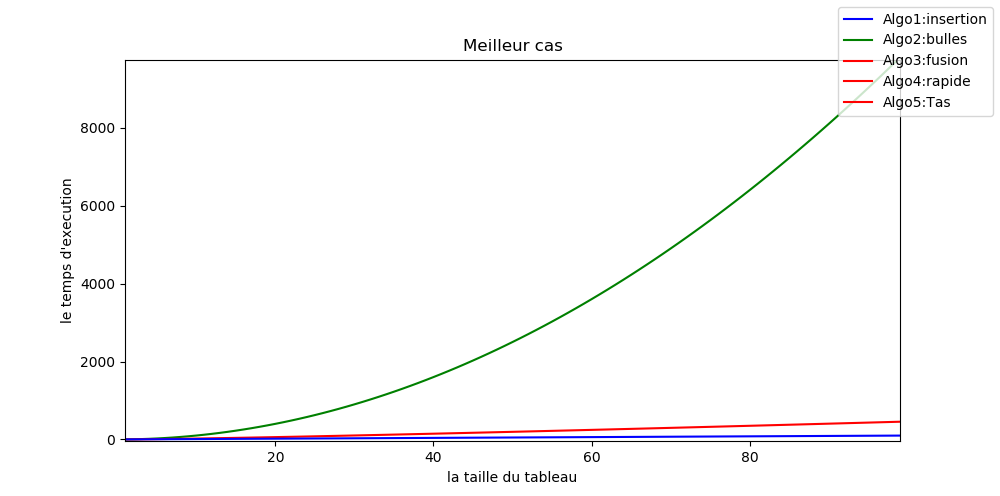
\includegraphics[width=1\textwidth]{graph/All_meilleur.png}
	

\subsubsection{Complexité expérimentale.}
1. Comparaison de la Complexité expérimentale dans le cas d'un tableau ordonné pour les cinq (5) algorithmes
	
		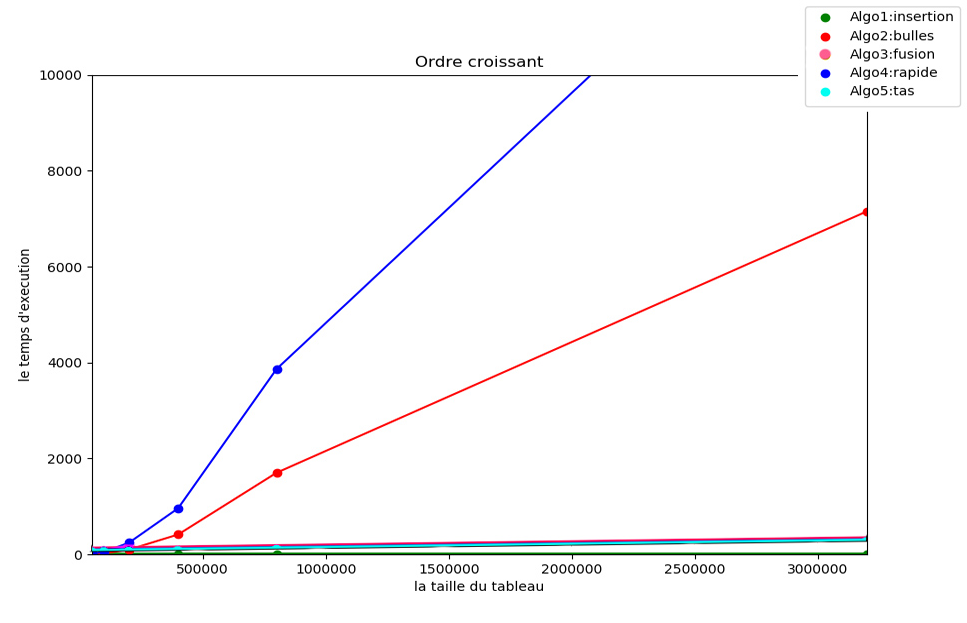
\includegraphics[width=1\textwidth]{graph/ordre_croissant.png}
	
2. Comparaison de la Complexité expérimentale dans le cas d'un tableau en ordre inverse pour les cinq (5) algorithmes
	
		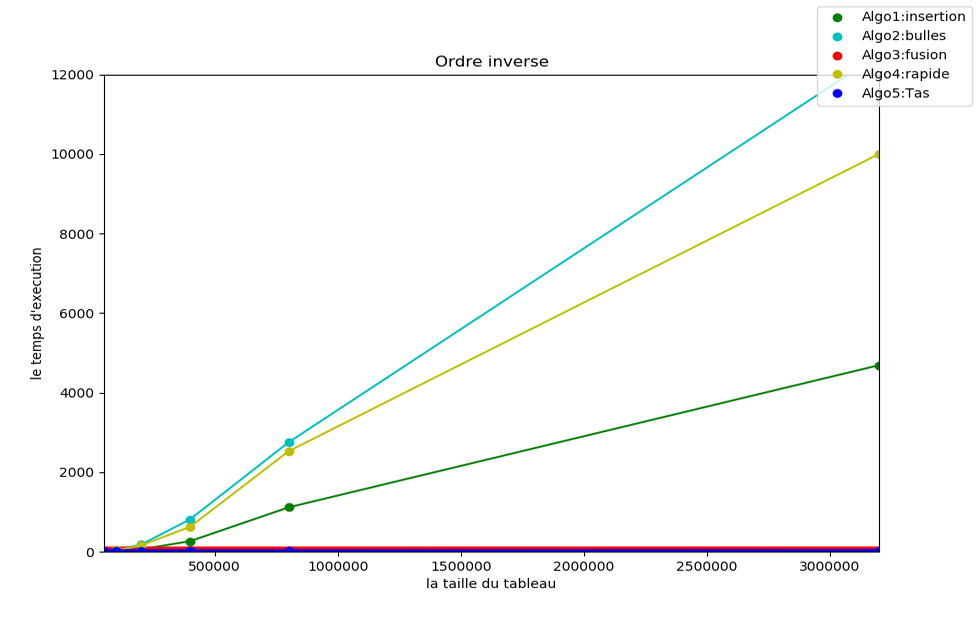
\includegraphics[width=1\textwidth]{graph/ordre_inverse.png}
	
3. Comparaison de la Complexité expérimentale dans le cas d'un tableau en ordre aléatoire pour les cinq (5) algorithmes
		
		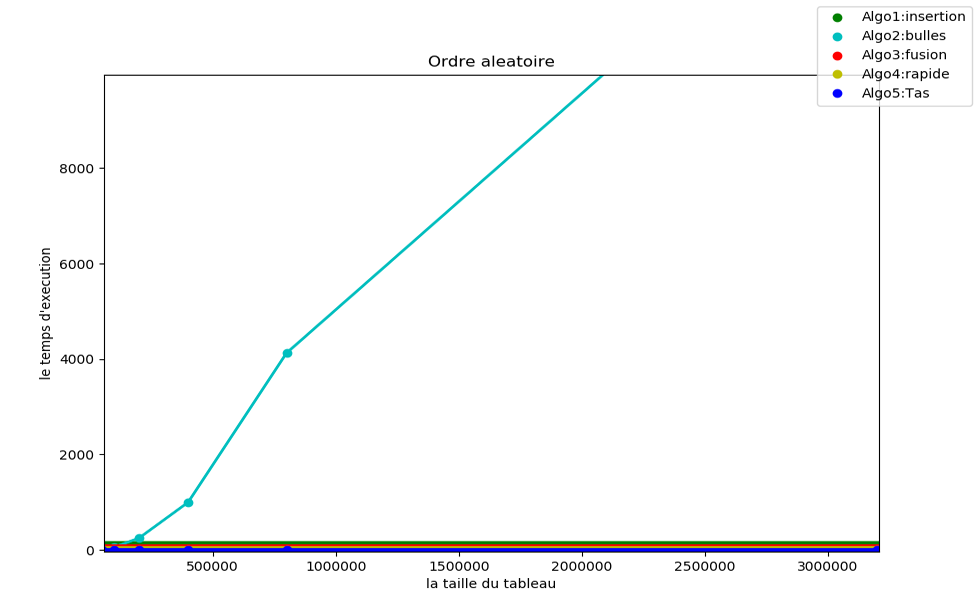
\includegraphics[width=1\textwidth]{graph/ordre_aleatoire.png}
		


\subsection{Tableaux comparatifs : des complexités et des temps d'exécution des cinq (5) algorithmes.}
\subsubsection{Complexité théorique.}
\begin{tabular}{|p{4cm}||p{4cm}|p{4cm}|}
\hline

Algorithme & Complexité au pire cas & Complexité au meilleur cas\\
\hline
Tri par insertion  & N² & N    \\
\hline
Tri à bulles  & N² & N² \\
\hline
Tri fusion  & N * $log_{2}$(N) & N * $log_{2}$(N) \\
\hline
Tri rapide & N² & N * $log_{2}$(N) \\
\hline
Tri par tas & N * $log_{2}$(N) & N * $log_{2}$(N) \\
\hline

\end{tabular}

\subsubsection{Temps d'exécution.}

1. Pire Cas\\

\begin{tabular}{|p{3cm}||p{2cm}|p{2cm}|p{2cm}|p{2cm}|p{2cm}|p{2cm}|}
\hline
Taille du Tableau (N) : & 50000 & 100000 & 200000 & 400000 & 800000  & 1600000\\
\hline
Tri par insertion  & 2.5*$10^{9}$ & $10^{10}$ & 4*$10^{10}$ & 1.6*$10^{11}$ & 6.4*$10^{11}$ & 2.56*$10^{12}$  \\
\hline
Tri à bulles  & 2.5*$10^{9}$ & $10^{10}$ & 4*$10^{10}$ & 1.6*$10^{11}$ & 6.4*$10^{11}$ & 2.56*$10^{12}$  \\
\hline
Tri fusion  & 540988,914 & 1151292,546 & 2441214,529 & 5159687,930 & 10873893,605 &  22856822,699\\
\hline
Tri rapide & 2.5*$10^{9}$ & $10^{10}$ & 4*$10^{10}$ & 1.6*$10^{11}$ & 6.4*$10^{11}$ & 2.56*$10^{12}$  \\
\hline
Tri par tas & 540988,914 & 1151292,546 & 2441214,529 & 5159687,930 & 10873893,605 &  22856822,699\\
\hline
\end{tabular}

\begin{tabular}{|p{3cm}||p{2.5cm}|p{2.5cm}|p{2.5cm}|p{2.5cm}|p{2.5cm}|}
\hline
Taille du Tableau (N) : & 3200000 & 6400000 & 12800000 & 25600000 &  51200000  \\
\hline
Tri par insertion  & 1.24*$10^{13}$ & 4.096*$10^{13}$ & 1.6384*$10^{14}$ & 6.5536*$10^{14}$ & 2.62144*$10^{15}$    \\
\hline
Tri à bulles  & 1.24*$10^{13}$ & 4.096*$10^{13}$ & 1.6384*$10^{14}$ & 6.5536*$10^{14}$ & 2.62144*$10^{15}$    \\
\hline
Tri fusion  & 47931716,376 & 100299574,709 & 209471433,329 & 436687434,481 & 908864004,608 \\
\hline
Tri rapide  & 1.24*$10^{13}$ & 4.096*$10^{13}$ & 1.6384*$10^{14}$ & 6.5536*$10^{14}$ & 2.62144*$10^{15}$    \\
\hline
Tri par tas & 47931716,376 & 100299574,709 & 209471433,329 & 436687434,481 & 908864004,608 \\
\hline
\end{tabular}\\




2. Meilleur cas\\

\begin{tabular}{|p{3cm}||p{2cm}|p{2cm}|p{2cm}|p{2cm}|p{2.05cm}|p{2cm}|}
\hline
Taille du Tableau (N) : & 50000 & 100000 & 200000 & 400000 & 800000  & 1600000\\
\hline
Tri par insertion  & 50000 & 100000 & 200000 & 400000 & 800000  & 1600000\\
\hline
Tri à bulles  & 2.5*$10^{9}$ & $10^{10}$ & 4*$10^{10}$ & 1.6*$10^{11}$ & 6.4*$10^{11}$ & 2.56*$10^{12}$  \\
\hline
Tri fusion & 540988,914 & 1151292,546 & 2441214,529 & 5159687,930 & 10873893,605 &  22856822,699\\
\hline
Tri rapide & 540988,914 & 1151292,546 & 2441214,529 & 5159687,930 & 10873893,6051 &  22856822,699\\
\hline
Tri par tas & 540988,914 & 1151292,546 & 2441214,529 & 5159687,930 & 10873893,605 &  22856822,699\\
\hline
\end{tabular}

\begin{tabular}{|p{3cm}||p{2.5cm}|p{2.5cm}|p{2.5cm}|p{2.5cm}|p{2.5cm}|}
\hline
Taille du Tableau (N) : & 3200000 & 6400000 & 12800000 & 25600000 &  51200000  \\
\hline
Tri par insertion  & 1.24*$10^{13}$ & 4.096*$10^{13}$ & 1.6384*$10^{14}$ & 6.5536*$10^{14}$ & 2.62144*$10^{15}$    \\
\hline
Tri à bulles & 1.24*$10^{13}$ & 4.096*$10^{13}$ & 1.6384*$10^{14}$ & 6.5536*$10^{14}$ & 2.62144*$10^{15}$    \\
\hline
Tri fusion  & 47931716,376 & 100299574,709 & 209471433,329 & 436687434,481 & 908864004,608 \\
\hline
Tri rapide & 1.24*$10^{13}$ & 4.096*$10^{13}$ & 1.6384*$10^{14}$ & 6.5536*$10^{14}$ & 2.62144*$10^{15}$    \\
\hline
Tri par tas & 47931716,376 & 100299574,709 & 209471433,329 & 436687434,481 & 908864004,608 \\
\hline
\end{tabular}


\subsection{Comparaison des cinq (5) Algorithmes.}

D'après les graphes et tableaux comparatifs ci-dessus nous pouvons passez à la comparaison entre les 5 algorithme5 de tri étudiés tout au long de ce projet, tel que chacun de ces algorithmes à des avantages et des inconvenants catégorisés en 3 parties : \\
\begin{enumerate}
	\item facilité d'implémentation.
	\item Temps d'exécution.
	\item Espace mémoire utilisé.\\
\end{enumerate} 
 pour ce qui est de l'espace mémoire nous ferons l'impasse dessus car, de nos jour on ne se souci pas de cet aspect, car la plupart des machines disposent de suffisamment d'espace mémoire.\\
 
 
puis pour la facilité d'implémentation il est claire que les algorithmes : \\
Tri pas Insertion et Tri à bulles  sont les plus instinctifs et donc les plus simples à implémenter.\\
Comparé aux trois autres qui demandent un peu plus de maitrise.\\

Enfin pour la rapidité d'exécution le tri par Insertion et tri à bulles ne sont pas très efficaces vu leurs complexités temporelles très élevées.\\
Quant au tri fusion il est nettement plus performant et donne de meilleurs résultats que les précédents algorithme, d'ailleurs il est encore largement utilisé notamment par les SGBD (pour les jointures entre tables par exemple).\\
Suivie du Tri rapide qui comme son nom l'indique est un tri assai rapide mais plusieurs variantes existent ainsi son efficacité dépend du choix du pivot, car si ce dernier est mal choisi on se retrouve avec un temps d'exécution similaire à celui des deux premiers algorithmes traités.\\

Puis viens le tri par tas qui est jusqu'au jour d'aujourd'hui considéré comme le plus intéressant des algorithme de tri , qui donne les meilleurs temps d'exécution!

\newpage

\section{Fonctions et procédure communes à tous les programmes}

\subsection{Fonction de création et de calcule du temps d'exécution de la fonction de tri pour un tableau comportant des données en ordre Croissant.}
\begin{sql}
double sortedTime(long int n) {
    
  long int *array = malloc(n*sizeof(long int));
  long int i;
  
  for (i = 0; i < n; i++)
  {
      array[i] = i;
  }
  clock_t start = clock();
  selectionSort(array, n); //replace with your function 
  clock_t end = clock();
  
  return (double) (end - start)/CLOCKS_PER_SEC;
}

\end{sql}

\subsection{Fonction de création et de calcule du temps d'exécution de la fonction de tri pour un tableau comportant des données en ordre inverse (décroissant). }
\begin{sql}
double inversedTime(long int n) {
    
  long int *array = malloc(n*sizeof(long int));
  long int i;
  
  for (i = 0; i < n; ++i)
  {
    array[i] = n - i;
  }
  clock_t start = clock();
  selectionSort(array, n); //replace with your function 
  clock_t end = clock();

  return (double) (end - start)/CLOCKS_PER_SEC;
}
\end{sql}

\subsection{Fonction de création et de calcule du temps d'exécution de la fonction de tri pour un tableau comportant des données en ordre Aléatoire.}
\begin{sql}
double randomTime(long int n) {
    
  long int *array = malloc(n*sizeof(long int));
  long int i;
  
  for (i = 0; i < n; ++i)
  {
    array[i] = (int) rand()%n;
  }
  clock_t start = clock();
  selectionSort(array, n); //replace with your function 
  clock_t end = clock();

  return (double) (end - start)/CLOCKS_PER_SEC;
}
\end{sql}

\subsection{Fonction de récupération des résultats des temps d'exécution dans un fichier.}
\begin{sql}
  void saveResults(double array[], long int n, char* name) {

     long int i;
     FILE * fp;
     fp = fopen ("tp3_results","a");
     fprintf(fp, name);
     fprintf(fp, "[");

     for(i = 0;i<n;i++) {
      fprintf(fp, "%lf, ",array[i]);
     }

     fprintf(fp, "]\n");
     fclose (fp);
  }
\end{sql}

\subsection{Programme MAIN de teste des fonctions et procédures.}
\begin{sql}
int main(int argc, char const *argv[])
{
	double *worstTimes = malloc(nbInputs*sizeof(double));
	double *bestTimes = malloc(nbInputs*sizeof(double));
	double *randomTimes = malloc(nbInputs*sizeof(double));
	int i;

	for (i = 0; i < nbInputs; i++)
	{
		worstTimes[i] = worstTime(inputs[i]);
		bestTimes[i] = bestTime(inputs[i]);
		randomTimes[i] = randomTime(inputs[i]);

	}

	saveResults(worstTimes,nbInputs, "worst case : ");
	saveResults(bestTimes,nbInputs, "best case : ");
	saveResults(randomTimes,nbInputs, "random case : ");

	return 0;
}

\end{sql}

\end{document}
